\documentclass[11pt,english]{tugasMIPA}

\usepackage{longtable}
\usepackage{ragged2e}
\usepackage{lipsum}
\usepackage{hyperref}
\hypersetup{
    colorlinks = true,
    citecolor  = {red},
    linkcolor  = {blue}
}
\usepackage{pdflscape}
\usepackage{tcolorbox}
\usepackage{enumitem}
\usepackage{multicol}
\usepackage{array}
\usepackage[margin=1cm]{caption}
\usepackage{listings}
\usepackage[T1]{fontenc}
\usepackage{tgbonum}
\usepackage{multicol}

%DEFINISI TAMBAHAN
\definecolor{sqlblue}{RGB}{0,90,160}
\definecolor{sqlgreen}{RGB}{0,128,0}
\definecolor{sqlgray}{RGB}{245,245,245}
\definecolor{sqlcomment}{RGB}{120,120,120}
\definecolor{sqlpurple}{RGB}{128,0,128}


\def\ojoin{\setbox0=\hbox{$\bowtie$}%
  \rule[-.02ex]{.25em}{.4pt}\llap{\rule[\ht0]{.25em}{.4pt}}}
\def\leftouterjoin{\mathbin{\ojoin\mkern-5.8mu\bowtie}}
\def\rightouterjoin{\mathbin{\bowtie\mkern-5.8mu\ojoin}}
\def\fullouterjoin{\mathbin{\ojoin\mkern-5.8mu\bowtie\mkern-5.8mu\ojoin}}

\lstdefinestyle{sqlstyle}{
    language=SQL,
    backgroundcolor=\color{sqlgray},
    basicstyle=\ttfamily\footnotesize,
    keywordstyle=\color{sqlblue}\bfseries,
    commentstyle=\color{sqlcomment}\itshape,
    stringstyle=\color{sqlgreen},
    numbers=none,
   % numberstyle=\tiny\color{gray},
  %  numbersep=6pt,
    showstringspaces=false,
    breaklines=true,
    frame=single,
    rulecolor=\color{gray!50},
    tabsize=2,
    captionpos=b,
    morekeywords={PRIMARY, KEY, FOREIGN, REFERENCES, UNIQUE, CHECK, DEFAULT, AUTO_INCREMENT, SERIAL, CASCADE, RESTRICT, INNER, LEFT, RIGHT, FULL, OUTER, JOIN, ON, GROUP, ORDER, BY, HAVING, LIMIT, OFFSET, AS, DISTINCT, BETWEEN, LIKE, IN, IS, NULL, AND, OR, NOT, BEGIN, COMMIT, ROLLBACK, TRANSACTION, INDEX, VIEW, CONSTRAINT}
}
\lstset{style=sqlstyle}

% ── Colors ───────────────────────────────────────────────────
\definecolor{ugmblue}{RGB}{0, 56, 101}
\definecolor{ugmgold}{RGB}{197, 155, 22}
\definecolor{lightgray}{RGB}{245, 245, 245}
\definecolor{sectionblue}{RGB}{0, 80, 140}
\definecolor{notegreen}{RGB}{34, 120, 60}
\definecolor{warnorange}{RGB}{200, 90, 0}
\tcbuselibrary{skins, breakable}

\newtcolorbox{infobox}[1]{
  colback=lightgray, colframe=ugmblue,
  fonttitle=\bfseries\color{white},
  coltitle=white, colbacktitle=ugmblue,
  title=#1, rounded corners, breakable
}

\newtcolorbox{warnbox}[1]{
  colback=red!10, colframe=warnorange,
  fonttitle=\bfseries,
  coltitle=white, colbacktitle=red!65,
  title=#1, rounded corners, breakable
}

\newtcolorbox{deliverablebox}{
  colback=green!5, colframe=notegreen,
  fonttitle=\bfseries,
  coltitle=white, colbacktitle=notegreen,
  title={Deliverables}, rounded corners, breakable
}
%Akhir DEFINISI Tambahan


%------------------------------------------------
% Awal Konten Utama Dokumen
%------------------------------------------------
\documenttype{Assignment on Lecture}
\coursename{Database Course}
\instructor{Khabib Mustofa}

\titleind{Relational Model and Query on It}
\fullname{Ahmad Kailani}
\idnum{21/530323/SPA/01010}
\level{Undergraduate} %appear in below part of the cover SARJANA/UNDERGRADUATE, MAGISTER/GRADUATE, or DOKTOR/POST GRADUATE
\program{Computer Science} %appear in below part of the cover
\yearsubmit{2026}

\begin{document}
%\input{coverTugas}
%\titlepageeng
\cover
\tableofcontents
\listoftables
\listoffigures
%\fontfamily{phv}\selectfont 
\clearpage
\pagenumbering{arabic}
\chapter{Guidelines and Assignment Format}
\begin{warnbox}{Academic Integrity}
\begin{center}
  All work submitted must be the result of the student's own thinking and work.
  Copying code or reports from other sources without clear attribution
  is a violation of academic integrity and will be subject to action in accordance
  with university regulations.
  \end{center}
\end{warnbox}
\section{Assignment Guidelines}
The assignment concerns the Relational Model and Queries on the Relational Model:
\begin{itemize}
    \itemsep0em
     \item Relational Algebra
     \item \textit{Structured Query Language (SQL})
\end{itemize}

The assignment answers are packaged in one chapter (chapter 2), whose sections have been provided in this template. The content of that chapter may be expanded as needed, but not reduced.

\begin{deliverablebox}{The assignment consists of four parts}
  \begin{enumerate}
    \itemsep0em
    \item Translate business requirements and processes into an ER diagram (\textit{Entity-Relationship Diagram}). The proposal must include an explanation of the ERD creation process
     \item Design and propose a relational database schema that aligns with the proposed ERD
     \item Given a query, propose a representation of the query in relational algebraic expressions.
     \item Propose a solution to the problem in the form of an SQL queries. If there are more than one possible query (with different operations or clauses), alternative queries must also be provided
\end{enumerate}
\end{deliverablebox}

Translated with DeepL.com (free version)

\begin{infobox}{Assignment Conditions}
\begin{enumerate}
    \itemsep0em
     \item The work may be done in groups with a maximum of 4 members.
     \item Each group member \textbf{must} contribute adequately, and master the material produced by their group.
     \item The work must be presented \textit{clearly, completely, and neatly, including the use of formal language that is easy to understand}
     \item The work must come from the team members' own thinking, and be agreed upon by all members
\end{enumerate}  
\end{infobox}

\section{Assignment Content Details}
\subsection{Case Domain}
It is desired to manage the academic data of a university with the following constraints:
\begin{infobox}{Process Constraints}
    \begin{itemize}
        \itemsep0em
     \item Every academic activity needs to be recorded transparently and preserve chronology/history
     \item The data storage design accommodates the following matters and processes:
     \begin{itemize}
         \itemsep0em \small
         \item A student is allowed to retake a course without any limit on the number of times
         \item The course grade (if retaken) used for the transcript is the \textbf{grade from the last attempt}
         \item Courses are either \textsc{Compulsory} or \textsc{Elective}.
         \item A course may have other courses as prerequisites
          \item A lecturer may teach a course in a semester in more than one class (parallel)
         \item Some courses may be offered in even or odd semesters
         \item A class for a course is taught entirely by one lecturer (not team teaching)
         \item The course grades and weights given are
         \begin{center}
         \begin{multicols}{2}
            \begin{tabular}{c|c}
             Grade & Weight \\ \hline
           A   & 4.00 \\
            A-  & 3.75 \\
            A/B & 3.50 \\
            B+ & 3.25 \\
            B & 3.00 \\ 
            B-  & 2.75 \\
         \end{tabular}  
         \columnbreak
         \begin{tabular}{c|c}
             Grade & Weight \\ \hline
            B/C  & 2.50 \\
            C+ & 2.25 \\
            C & 2 \\
            C/D & 2.5 \\
            D & 1.00 \\ 
             D & 0.00 \\ 
         \end{tabular} 
         \end{multicols}
         \end{center}
         \item The formula for calculating GPA from $n$ courses is:
         \[GPA = \frac{\sum_{i=1}^{n}{{\text{credits}}_i.{\text{weight}}_i}}{\sum_{i=1}^{n}{{\text{credits}}_i}}\]
     \end{itemize}
    \end{itemize}
\end{infobox}

\subsection{Output/Outcome of the Assignment}
The following are some \textbf{minimal} output/outcome to be addressed.

\begin{deliverablebox}
    \begin{enumerate}
        \itemsep0em
     \item An E-R diagram (ERD) that matches the points above! (starting from identification: entities, relations, cardinalities, etc.)
     \item A complete schema of the database tables that matches the ERD created; for example in the form \newline \texttt{Student(nim, name, gender, studyProgram,\dots) \newline Lecturer(nip, \dots)}
     
     And \textbf{also SQL DDL commands} for defining the tables above (complete with all \textit{constraints})!
     \item DML commands for the questions below:
     \begin{enumerate}
         \itemsep0em \footnotesize \bfseries
         \item List of elective course names and the courses that are their prerequisites (only name and course code information is sufficient). Courses that do not have prerequisites should still be displayed!
         \item List of elective courses taken by Computer Science students of the '2024' cohort in the odd semester of academic year 2026/2027!
         \item List of favorite elective courses for Computer Science students, namely the three courses with the most enrollees in the last three years!
         \item List of students who have a Semester Grade Point Average for the odd semester of 2025/2026 of no less than 3.25! (understand the difference between Semester GPA and Cumulative GPA)
         \item List of students and the Cumulative GPA they have obtained to date! (courses that have been retaken only need to be counted once) 
     \end{enumerate}
     \item Relational algebra expression for each given query!
    \end{enumerate}
\end{deliverablebox}

\vspace{.2cm}
For each query above, the steps for working on it need to be described:
\begin{enumerate}
    \itemsep0em
     \item identify the tables that need to be involved
     \item determine the join criteria and join type: \textsc{inner join, natural join, left/right join} or \textsc{outer join}
     \item Valid SQL commands. If a \textsc{VIEW} is needed as a temporary table, please also write it out in order.
     \item if there is more than one \textit{equivalent} SQL query, it will be a bonus if you can also write that query!
\end{enumerate}

\section{Sample Problem and Its Solution}
Suppose the following query is given:
\begin{tcolorbox}{}
\begin{quote}
    \textit{Display the list of elective courses that have never been taken/attended by students}
\end{quote}
\end{tcolorbox}
then an example answer is as follows:
\begin{infobox}{Query number 1}
    \begin{enumerate}
        \itemsep0em \small
         \item \textbf{Tables needed in the query:} \textsc{Course (Mk), CourseEnrollment (Pk)}
         \item if using the SET DIFFERENCE operation there is no join process, so there is no join criterion. As an alternative, LEFT JOIN can be used, with the criterion \texttt{Mk.courseId= Pk.courseId} %\newpage
         \item \textbf{The required query} 
         \begin{lstlisting}[caption= SET DIFFERENCE approach]
SELECT * FROM Course Mk WHERE (type='E') and courseId NOT IN 
    (SELECT courseId FROM CourseEnrollment Pk)       
         \end{lstlisting}
         \item Equivalent SQL alternatives
         \begin{lstlisting}[caption=Using LEFT JOIN]
SELECT Mk.* FROM Course Mk LEFT JOIN CourseParticipant Pk ON (Mk.courseId=Pk.courseId) 
    WHERE Mk.type='E' and Pk.courseId is NULL
         \end{lstlisting}
      \begin{lstlisting}[caption=Using EXISTS]
SELECT * FROM Course Mk WHERE (type='E') and 
    NOT EXISTS
    (SELECT courseId FROM CourseEnrollment Pk 
        WHERE Pk.courseId=Mk.courseId)       
         \end{lstlisting}  
 \item Proposed Relational algebra expression
 
 \[
\begin{array}{c}
(\pi_{\text{courseId}}(\sigma_{\text{type='E'}}\left(\text{Course}) \right) - \\ \pi_{\text{courseId}}\left(\text{Course}\right))   \bowtie \text{Course}
\end{array}
 \]


 \[
 \begin{array}{c}
DIFF1 \leftarrow \pi_{\text{courseId}}(\sigma_{\text{type='E'}}\left(\text{Course}) \right)\\
 DIFF2 \leftarrow (DIFF1 - \pi_{\text{courseId}}\left(\text{Course}\right))  \\
DIFF2 \bowtie \text{Course}
 \end{array}
 \]
 
    \end{enumerate}
\end{infobox}
\chapter{Results and Discussion}
\begin{tcolorbox}[title=Group Members]
    \begin{enumerate}
        \itemsep0em
        \item Nashwan Hafid Andayuri, 25/554944/PA/23251
        \item Mhs 2, NIM: 
        \item Mhs 3, NIM:
    \end{enumerate}
\end{tcolorbox}
\section{Entity Relationship Diagram}
From the analysis of the business processes and the given constraints, this section can explain several things, including: \textit{cardinality mapping}, relevant attributes and keys, etc.

The ER diagram for the Academic Database is shown in Figure \ref{gb:1}
\begin{figure}[!h]
    \centering
    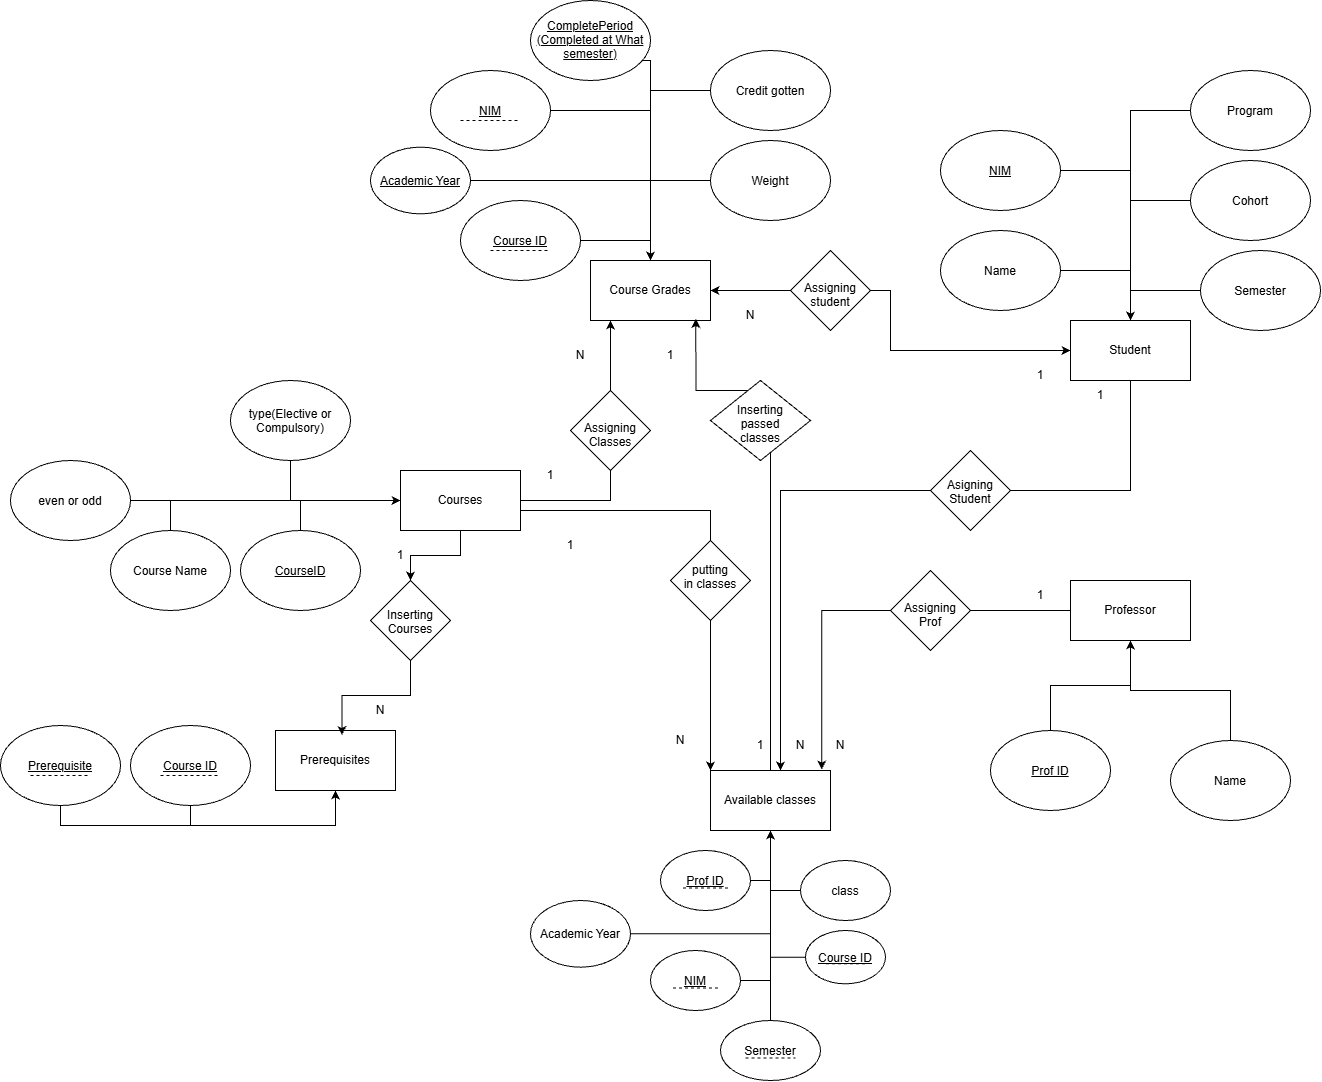
\includegraphics[width=.85\linewidth]{ERD.png}
    \caption{ER Diagram of the Academic Database}
    \label{gb:1}
\end{figure}
\section{Schema of Tables in the Database}
\begin{tcolorbox}[title=Table Schema in the Academic Database]
\begin{itemize}
    \itemsep0em
     \item \texttt{students(nim, name, semester, cohort, program)}
     \item \texttt{professors(prof id, name)}
      \item \texttt{courses(course name, course id, period, type, academic year)}
      \item \texttt{prerequisites(prerequisite, course id)}
      \item \texttt{AvailableClasses(prof id, nim, class, course id, semester, academic year)}
      \item \texttt{CourseGrades(course id, nim, academic year,completed period, credits, weight)}
      \item \texttt{CREATE TABLE students (
      	nim VARCHAR(20) PRIMARY KEY,
      	name VARCHAR(100) NOT NULL,
      	semester INT,
      	cohort VARCHAR(20),
      	program VARCHAR(100)
      	);
      	
      	CREATE TABLE professors (
      	prof_id VARCHAR(20) PRIMARY KEY,
      	name VARCHAR(100) NOT NULL
      	);
      	
      	CREATE TABLE courses (
      	course_id VARCHAR(20) PRIMARY KEY,
      	course_name VARCHAR(100) NOT NULL,
      	period VARCHAR(20),
      	type VARCHAR(50),
      	academic_year VARCHAR(20)
      	);
      	
      	CREATE TABLE prerequisites (
      	prerequisite VARCHAR(20),
      	course_id VARCHAR(20),
      	PRIMARY KEY (prerequisite, course_id),
      	FOREIGN KEY (prerequisite) REFERENCES courses(course_id),
      	FOREIGN KEY (course_id) REFERENCES courses(course_id)
      	);
      	
      	CREATE TABLE AvailableClasses (
      	prof_id VARCHAR(20),
      	nim VARCHAR(20),
      	class VARCHAR(20),
      	course_id VARCHAR(20),
      	semester INT,
      	academic_year VARCHAR(20),
      	PRIMARY KEY (prof_id, class, course_id, semester, academic_year),
      	FOREIGN KEY (prof_id) REFERENCES professors(prof_id),
      	FOREIGN KEY (nim) REFERENCES students(nim),
      	FOREIGN KEY (course_id) REFERENCES courses(course_id)
      	);
      	
      	CREATE TABLE CourseGrades (
      	course_id VARCHAR(20),
      	nim VARCHAR(20),
      	academic_year VARCHAR(20),
      	completed_period VARCHAR(20),
      	credits INT,
      	weight DECIMAL(3, 2),
      	PRIMARY KEY (course_id, nim, academic_year),
      	FOREIGN KEY (course_id) REFERENCES courses(course_id),
      	FOREIGN KEY (nim) REFERENCES students(nim)
      	);}
     
\end{itemize}  
\end{tcolorbox}
\section{Business Questions and Solutions Using SQL}
\subsection{Question number 1}
\begin{tcolorbox}
  \textit{List of elective course names and the courses that are their prerequisites (only name and course code information is sufficient). Courses that do not have prerequisites should still be displayed!}  
\end{tcolorbox}
\begin{enumerate}
    \itemsep0em
    \item Tables needed to answer the query:
    \item Join criteria (if any)
    \item SQL command according to the question
    \begin{lstlisting}
SELECT * FROM course where type='E'
    \end{lstlisting}
    \item Alternative SQL commands (if any) with adequate explanation
\end{enumerate}

\subsection{Question number 2}
\begin{tcolorbox}   
List of elective courses taken by Computer Science students of the '2024' cohort in the odd semester of academic year 2026/2027!
\end{tcolorbox}
\begin{enumerate}
    \itemsep0em
    \item Tables needed to answer the query:
    \item Join criteria (if any)
    \item SQL command according to the question
    \begin{lstlisting}
SELECT 
    FROM
    \end{lstlisting}
    \item Alternative SQL commands (if any) with adequate explanation
\end{enumerate}

\subsection{Question number 3}
\begin{tcolorbox}
    List of favorite elective courses for Computer Science students, namely the three courses with the most enrollees in the last three years!
\end{tcolorbox}
\begin{enumerate}
    \itemsep0em
    \item Tables needed to answer the query:
    \item Join criteria (if any)
    \item SQL command according to the question
    \begin{lstlisting}
SELECT 
    FROM
    \end{lstlisting}
    \item Alternative SQL commands (if any) with adequate explanation
\end{enumerate}

\subsection{Question number 4}
\begin{tcolorbox}
List of students who have a Semester Grade Point Average for the odd semester of 2025/2026 of no less than 3.25! (understand the difference between Semester GPA and Cumulative GPA)
\end{tcolorbox}
\begin{enumerate}
    \itemsep0em
    \item Tables needed to answer the query:
    \item Join criteria (if any)
    \item SQL command according to the question
    \begin{lstlisting}
SELECT 
    FROM
    \end{lstlisting}
    \item Alternative SQL commands (if any) with adequate explanation
\end{enumerate}

\subsection{Question number 5}
\begin{tcolorbox}
    List of students and the Cumulative GPA they have obtained to date! (courses that have been retaken only need to be counted once) 
\end{tcolorbox}
\begin{enumerate}
    \itemsep0em
    \item Tables needed to answer the query:
    \item Join criteria (if any)
    \item SQL command according to the question
    \begin{lstlisting}
SELECT 
    FROM
    \end{lstlisting}
    \item Alternative SQL commands (if any) with adequate explanation
\end{enumerate}
\cleardoublepage
\addcontentsline{toc}{chapter}{\refname}
\bibliography{pustaka.bib}
\end{document}
